\chapter{Background Research}\label{ch:backgroundresearch}
This chapter introduces the theories about augmented reality and human depth perception on which this project is based, as well as presents some reflections about the relation between the two. Lastly, a description of the state of the art provides some examples of existing systems with similar goals as those this project aims toward.

\section{Visual Depth Perception Within Humans}
Mathematical depth is to be thought of as the third dimension (first and second being length and width respectively). Depth is measured as the distance between two points in a vertical upward/downward and horizontal inward/outward direction depending on the objects of attention as well as angle of view (AOW) \cite{Gale}. Perception on the other hand defines the brain’s ability to sense and be aware of objects' existence through one or more of the five human senses: Hearing, smell, taste, touch, and vision. Of these the sense of vision --- primarily processed in the brain’s occipital lobe based on signals received from photoreceptors on the eyes’ retina registering the spatial, temporal, and chromatic components of light \cite{Spector2003} --- is considered the primary but not sole sense for perceiving depth. As \textit{The Gale Encyclopedia of Science} states: \textit{“While depth perception results primarily from our sense of vision, our sense of hearing also plays a role.”} \cite{Gale}. Research with infants has further revealed that the ability to perceive depth visually within humans exists from as early on as two month of age \cite{Gale}. Thus it follows that visual depth perception within humans can be defined as the ability for humans with normal functioning eyes to use sight to see in three dimensions and estimate the spatial distance between objects (including distance to oneself). As has been mentioned in Chapter \ref{ch:problemstatement}, an AR application is developed during this project, the implementation of which is described in Chapter \ref{ch:implementation}. The following sections describe various depth cues, and discuss how it will be relevant to the design of the application.

\subsection{Depth cues}
For the brain to determine an object’s location in space and its relation to other objects, certain estimates referred to as cues are used. Overall the cues can be separated into one of two types, namely monocular and binocular cues, based on single eye and two eye information respectively. Furthermore, the monocular cue can be subdivided into pictorial cues and non-stereoscopic cues. To the pictorial cues belongs: Interposition, shading and lighting, aerial perspective, elevation, linear perspective, texture gradients, and retinal size, while the non-stereoscopic cues consist of motion parallax and accommodation. Meanwhile, members to the binocular cues are convergence and retinal disparity \cite{Gale}. For this project, the AR application will only rely on monocular cues, as the typical smartphone is equipped with a non-stereo camera. Therefore, binocular cues will not be discussed. 

\subsubsection{Monocular Depth Cues}
The following explains the aforementioned cues connected to monocular vision, meaning that these cues require access to information from only one eye in order to be perceived.

\textit{Interposition} is when one object appears to be partially blocked by another object as seen in Figure \ref{fig:cue0}). It is also referred to as occlusion or overlapping. During the image processing done by the brain this cue is used to determine which object should be perceived as the closest to the viewer since objects nearer the viewer tends to cover up parts of objects further behind \cite{Gale}. Interposition is utilised in the application, as the edge of the virtual hole through which users look occludes certain parts of the model. This is described in further detail in Chapter \ref{ch:implementation}.

\begin{figure}[h!]
   \centering
   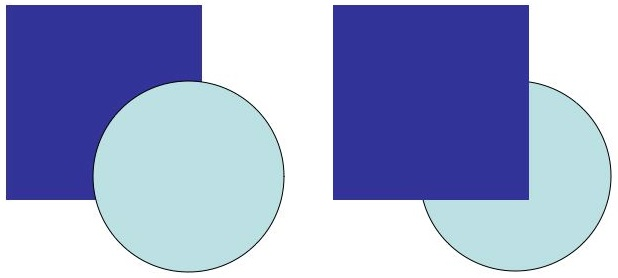
\includegraphics[width=0.6\textwidth]{figures/cue0.jpg}
   \caption{Interchange in occluded object to showcase the effect of interposition \cite{Heeger}}\label{fig:cue0}
\end{figure}

\textit{Shading and lighting} cues clue to the distance between the object and a light source as the surface closest to the light appears brighter than that of the surfaces further away, which gradually darkens by the distance from the light source. Moreover, surfaces turned away from the light are perceived as dark progressing towards black the nearer they are to the light source. The viewer uses this to estimate whether to perceive the object as more convex or concave in shape \cite{Gale}. Shading an lighting is utilised in the application to a slight degree, as the shape of the model is made clearer by the lighting.

\begin{figure}[h!]
   \centering
   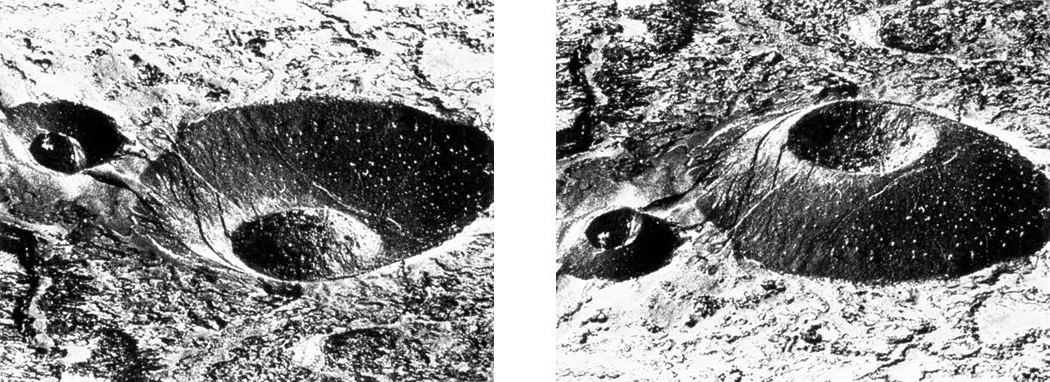
\includegraphics[width=0.8\textwidth]{figures/cue1.jpg}
   \caption{Effects on the human depth perception by variations in shading and lighting \cite{Heeger}}\label{fig:cue1}
\end{figure}

\textit{Aerial perspective}, also known as \textit{atmospheric perspective},  involves the sharpness of an object. From this it follows that the sharper an object is perceived by the eye, the nearer to the viewer the said object is interpreted to be, and vice versa. An example can be seen in Figure \ref{fig:cue2} The cause of this effect is the particles in the atmosphere e.g. water vapour and dust which either scatter or absorb light reflected by an object \cite{Gale}. This is not implemented in the application, as this cue is mostly relevant to convey large distances, which will not be necessary in this project.

\begin{figure}[h!]
   \centering
   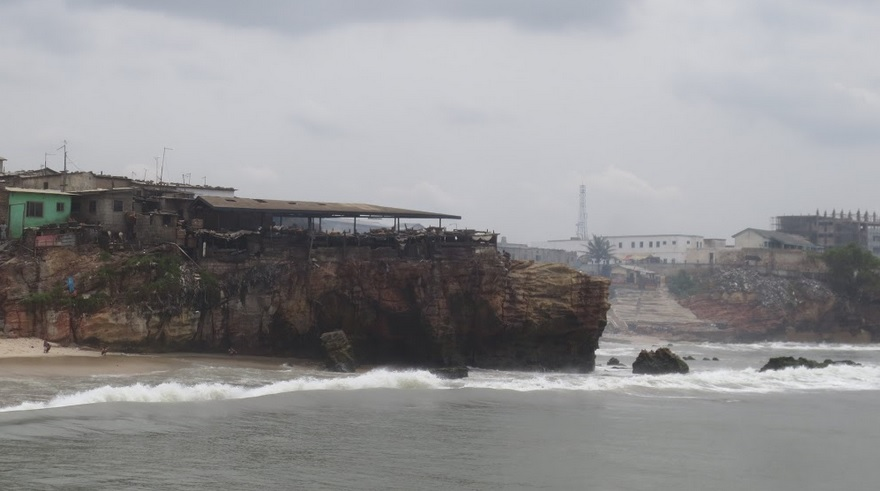
\includegraphics[width=0.8\textwidth]{figures/cue2.jpg}
   \caption{Example of aerial perspective---the buildings to the left are closer than the buildings to the right}\label{fig:cue2}
\end{figure}

\pagebreak
\textit{Elevation} considers the eyes' placement of an object in correlation to the horizontal line, as can be seen in Figure \ref{fig:cue3}. Here the horizon (horizontal line, Figure \ref{fig:cue3}) is observed as either higher (foreground 1, Figure \ref{fig:cue3}) or lower  (foreground 2, Figure \ref{fig:cue3}) than that of the foreground. Thus objects placed near to the horizon are perceived as being farther away in contrast to objects located near either the upper or lower outline of the visual field which are perceived to be nearer the viewer \cite{Gale}.

\begin{figure}[h!]
   \centering
   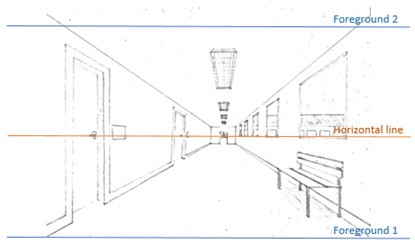
\includegraphics[scale=0.85]{figures/cue3.jpg}
   \caption{An example of elevation}\label{fig:cue3}
\end{figure}

\textit{Linear perspective} is the correlation occurring between the decrease in an object’s size and the separating spaces between objects when repeatedly positioned along a line and the perceived increase in distance from the point of view (POV) until the vanishing point is reached where the objects cease to be visible, as can be seen in Figure \ref{fig:cue4} \cite{Gale}. Both elevation and linear perspective are utilised in this project; several lines in the model go towards a vanishing point, and parts of the model are placed closer to the viewer than others, thus serving as the foreground.

\begin{figure}[h!]
   \centering
   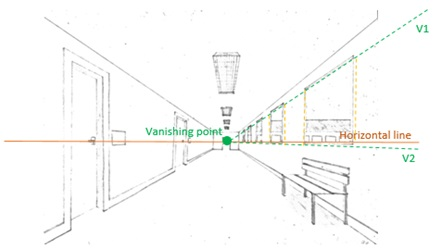
\includegraphics[scale=0.85]{figures/cue4.jpg}
   \caption{An example of linear perspective}\label{fig:cue4}
\end{figure}

\textit{Texture gradients} concern the effect of texture perception by an increase in distance. With increased distance the size of elements making up the surface texture appear to be smaller while the distance between said elements seems to decrease, as seen in Figure \ref{fig:cue5} \cite{Gale}. For instance, the model used in the application has a brick texture, and the bricks appear smaller the further they are from the viewer.

\begin{figure}[h!]
   \centering
   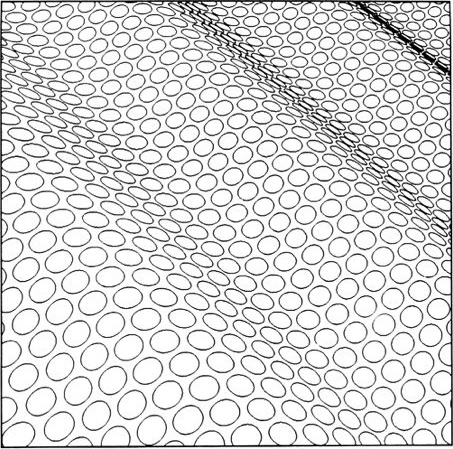
\includegraphics[width=0.4\textwidth]{figures/cue5.jpg}
   \caption{Texture gradient \cite{Heeger}}\label{fig:cue5}
\end{figure}

\textit{Retinal size} considers how the brain automatically distinguishes between an object being distant or near. This is interpreted based on the retinal image recognition of an object as small or large respectively. It is utilised in case of the absence of additional visible cues to suggest the opposite. Thus, as it can be seen in Figure \ref{fig:cue6} the dotted arrow A, although having the same size as the arrow B, looks larger when comparing the projections of A and B on the retina,  hence it is considered to be nearer. However, as can be seen from the two air planes in Figure \ref{fig:cue7} this method for distinguishing distance only applies for objects of the same size since a larger object located farther away may look the same size on the retina if compared to a nearer small object \cite{Gale}. This is not a cue consciously used in the project.

\begin{figure}[h!]
   \centering
   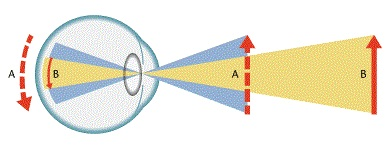
\includegraphics[scale=0.7]{figures/cue6.jpg}
   \caption{Retinal size used to infer distance \cite{Perslides}}\label{fig:cue6}
\end{figure}

\begin{figure}[h!]
   \centering
   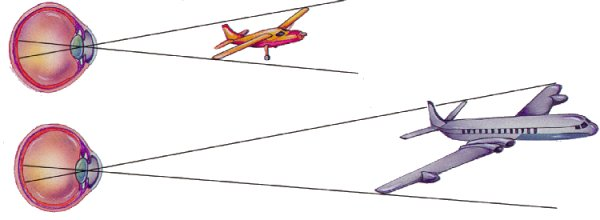
\includegraphics[scale=1]{figures/cue7.jpg}
   \caption{Retinal size, wrong interpretation of reality \cite{Psych}}\label{fig:cue7}
\end{figure}

\textit{Motion parallax} is the perception of apparent motion of two stationary objects with relative different distances to the viewer (located respectively in front of and behind of the viewer’s fixation point) caused by changes in the viewer’s position. Objects relatively close to the viewer is perceived as moving at a higher speed when compared to objects located in the distance. The near object will also seem to be moving in the opposite direction as the viewer whereas the farther away object will be heading in the same direction as the viewer, as illustrated in Figure \ref{fig:cue8} and \ref{fig:cue9}. In addition to this it is also noticeable that distant objects seem to move smaller distances than that of objects near the viewer \cite{Gale} \cite{Shrestha2013} \cite{Skybrary}. Motion parallax is utilised in this project, since users may choose to move "around" the model, causing the foreground to appear to move at a different pace than the parts of the model which are further away.

\begin{figure}[h!]
	\centering
	\begin{subfigure}[h!]{0.45\textwidth}
		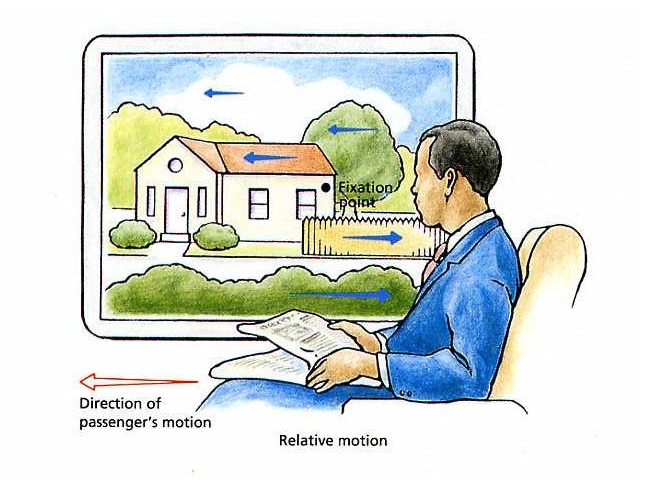
\includegraphics[width=\textwidth]{figures/cue8.jpg}
		\caption{Experiencing motion parallax \cite{Parallax0}}\label{fig:cue8}
	\end{subfigure}
	\begin{subfigure}[h!]{0.45\textwidth}
		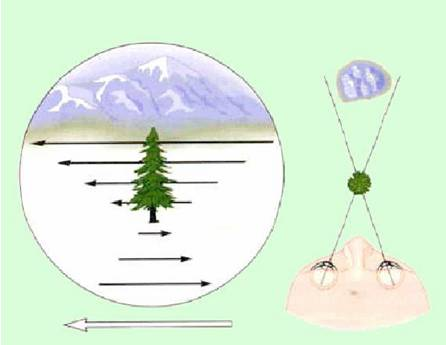
\includegraphics[width=\textwidth]{figures/cue9.jpg}
		\caption{Motion parallax explained \cite{Skybrary}}\label{fig:cue9}
	\end{subfigure}
	\caption{Illustrations demonstrating motion parallax}
\end{figure}

\textit{Accommodation} is the physiological changes happening to the lens’ curvature to sharpen the retinal images of near and far objects. In order to have the eye focus on a distant object the lens have to flatten (Figure \ref{fig:cue10}, left). Meanwhile, to focus on near objects the lens becomes more of a curve (Figure \ref{fig:cue10}, right). These changes in the lens’ curvature are controlled by the ciliary muscle which seemingly sends signals as feedback to the brain about alterations in the muscle tension that may assist in determining the distance to the object \cite{Gale}. Accommodation is not utilised in this project, as users will be looking at a two-dimensional projection of a virtual 3D model. For accommodation to be properly implemented, the software would have to track where on the model users are looking and adjust the focus accordingly.

\begin{figure}[h!]
   \centering
   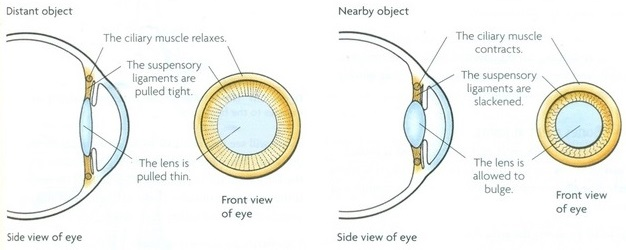
\includegraphics[width=\textwidth]{figures/cue10.jpg}
   \caption{Accommodation, left: Distant focused lens, right: Near focused lens \cite{Biology2014}}\label{fig:cue10}
\end{figure}

In addition to monocular cues comes the semi-cue: \textit{Familiarity} which is used in other sections of humans’ visual processing as well. This takes as its starting point an individual’s previous experience with the spatial characteristics of various objects and contributes to determine the distance to the object thereby assisting in the spatial perception \cite{Gale}. This is not utilised in this project, but may have affected how the size of the model is perceived, as will be discussed in Chapter \ref{ch:implementation}.

\subsection{Reflections Upon Human Depth Perception in The Context of AR}
A major part of an AR system is to have the digital 2D overlay image appear as an integrated part of the real world environment generated by the real time video transmission. Cameras imitate the eye’s retina in the way it produces its images, see Figure \ref{fig:camera}. Thus it befalls that the retina based cues for depth perception in the human eye also applies to a camera’s way of processing the sense of depth in an image.

\begin{figure}[h!]
   \centering
   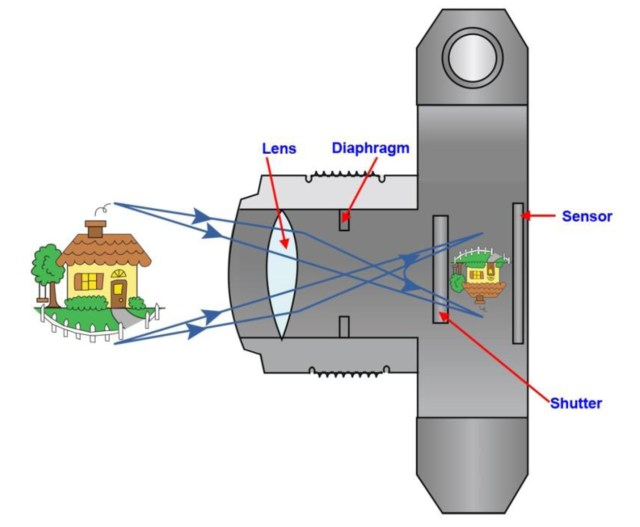
\includegraphics[width=0.5\textwidth]{figures/camera.jpg}
   \caption{Camera image production \cite{Camera}}\label{fig:camera}
\end{figure}

To this it has to be added that unless two cameras are used to produce the image, one only have to consider the monocular depth cues, given that the binocular cues requires two eyes, or in this case two cameras, in order to be obtained. This further means that the pictorial depth cues become the primary source for integrating a digital AR overlay into real time footage, since the non-stereoscopic monocular depth cues relate to physical movement or changes in the eye muscles, meaning they are outside the AR system’s control.

\textit{Augmented reality for underground infrastructure: the problem of spatial perception} is a research study from 2011 done into the usage of AR for underground infrastructure in regard to the spatial perception \cite{Cote2011}. This research showed the relevancy of having the virtual data of the AR extension displayed in a visually clear and meaningful way. It further showed the significance of providing good depth perception in AR applications, especially when the goal is to display subterranean items elsewise concealed (in their case underground pipes). This is because the depth cues help the mind understand that the items are to be perceived as being underground. The researcher's solution to resolve this was to have the pipes shown in a “virtual hole” (see Figure \ref{fig:pipes0}), since the way the brain is used to see items situated underground is by excavations (the hole) and it therefore understands this kind of scene immediately. As the AR application for this project will also convey an underground structure, it follows that depth cues are important to incorporate into the design so that users may understand the spatial relation between the real world and the virtual model.

\begin{figure}
	\centering
	\begin{subfigure}[h!]{\textwidth}
		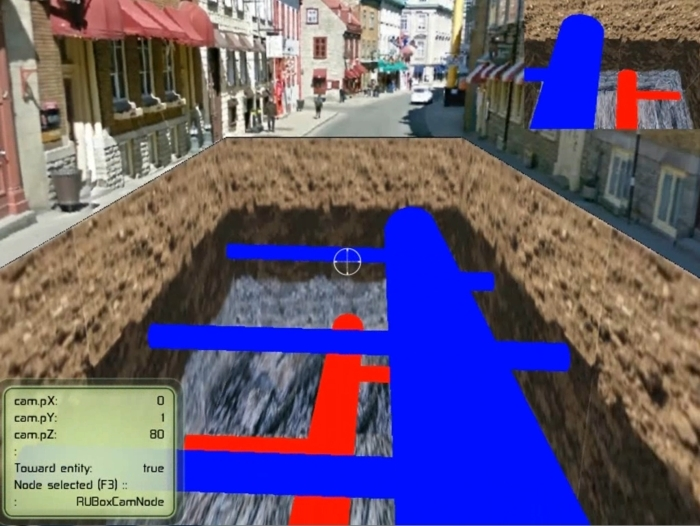
\includegraphics[width=\textwidth]{figures/pipes_0.jpg}
		\caption{Untextured}\label{fig:pipes0}
	\end{subfigure}
	\begin{subfigure}[h!]{\textwidth}
		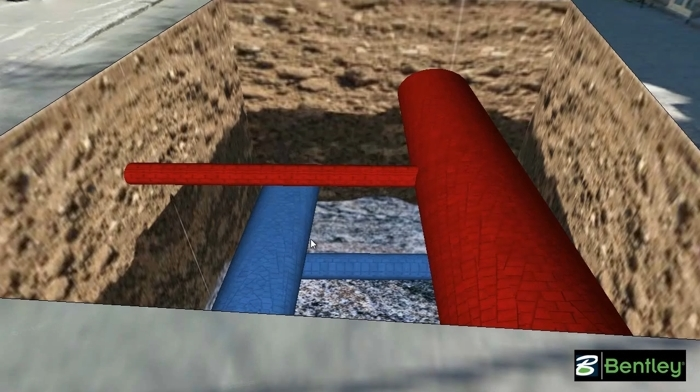
\includegraphics[width=\textwidth]{figures/pipes_1.jpg}
		\caption{Textured}\label{fig:pipes1}
	\end{subfigure}
	\caption{Virtual underground pipes \cite{Cote2011}}
\end{figure}

Half a year later in the blog post under the headline:\textit{Augmented reality for subsurface utilities: Further improving perception} the original concept has gone through a redesign to improve the depth perception. In this version the original uniform colour of the pipes was replaced with textures, and a source light which changes the reflections (shading) along the surfaces was added as well. This was all done in order to give the pipes a more 3D looking shape compared to the original, see Figure \ref{fig:pipes1} \cite{Cote2011}. Likewise, the model used in the application for this project contains textures and light sources, as it would be difficult for users to perceive the depth of a model with solid colour.

\section{Augmented Reality}\label{sec:background_ar}
As suggested by Madden, AR is to be thought of as the opposite of Virtual Reality (VR). As Madden explains it: “Virtual reality immerses the user in a computer-generated world whereas AR combines the real world with computer graphics.” \cite{Madden2011}. Moreover, Madden points out that where it requires the user to acquire special equipment to experience VR, AR requires only a device able to capture the environment (e.g. a smartphone or tablet) as well as methods to experience the computer world, typically in the form of an overlaying computer graphic in the camera window \cite{Madden2011}. Based on this, Madden defines AR as a technology which combines the real world with computer graphics, tracking and/or providing interaction with objects in real-time. Furthermore, AR provides recognition of images or objects, as well as delivering real-time context or data. By utilising this definition Madden allows technologies to be included that are not considered AR in the strictest interpretations e.g. AR browsers \cite{Madden2011}.

In relation to the above definition of AR, Madden makes a distinction between two tracking systems, namely tracking by markers and markerless tracking. The method of tracking by markers makes use of patterned images which activate a certain action when recognised. Examples of markers are the fiduciary marker, Quick response codes (QR), and Microsoft Tags. Markerless tracking on the other hand works by tracking objects in the real world not using markers made for the purpose. An example of markerless tracking is facial recognition \cite{Madden2011}.

Approaches to mobile AR are mainly split into two paths, namely AR using location and orientation data to compute what is viewed, and AR using actual image content captured by a camera to compute what is viewed referred to as \textit{computer vision}.

As introduced by Madsen and Lal \cite{Lal2010}, AR can be associated with three major challenges:

\begin{itemize}
\item Camera tracking 
\item Handling occlusions
\item Illumination consistency
\end{itemize}

The challenge with camera tracking involves \textit{“matching position and orientation of the camera to the coordinate system of the scene”} \cite{Lal2010}, which deals with making sure the angle of the scene captured by the camera matches that of the virtual scene. Handling occlusions means \textit{“having sufficient 3D information of the real scene to handle occlusion between real and virtual geometry”} \cite{Lal2010}, so that real-world objects such as people walking by may occlude the virtual objects. Lastly, illumination consistency deals with the problems of \textit{“having sufficient knowledge of the real scene illumination to be able to render virtual objects with scene consistent illumination, including shadows”} \cite{Lal2010}. The latter of these three is especially important for creating visually credible AR in outdoor environments because of this scenario’s dynamically changing illumination.

\subsection{Tracking Systems} \todo{this next subsection needs to have all the sources added} 
When dealing with AR one of the more important choices to be made in regards to the system design, is the selection of a suitable tracking system, since these all comes with their advantages and disadvantages. As mentioned before approximately three different types of tracking systems exist: The location/orientation based system utilising GPS and gyroscopic data, the marker based system using pattern recognition for tracking, and the markerless system that tracks by processing environmental data.    

\subsubsection{Location and Orientation Based Tracking Systems}
This form of tracking is the simplest form. For this tracking system the system uses sensors like the GPS and gyroscope to gather coordinate information about the user’s current position and orientation. From this it calculates where to insert the AR overlay. The pros of this tracking system is that it is robust. However, it only works for providing more general knowledge like background information about the visited location, direction guidance, and other similar aspects that does not need to accurately match into the real world to be experienced \cite{Woodford}.

\subsubsection{Fiducial Marker Tracking Systems} \todo{new sources in this section}
Tracking systems using fiducial markers, e.g. QR codes, can be thought of as an advanced form of barcode scanning. The process for detecting fiducial markers can in general be split into two steps. First step is \textit{Detecting Candidates}. In this step an adaptive threshold is used to segment the black squares defining the marker. From the segmentation contours are extracted. Through this process all concave contours are eliminated such that only contours indicating a square are accepted. Then in the second and final step, \textit{Verifying Candidates}, the potential candidates are verified. This is done by having each candidate checked for internal codification, which involves a perspective transformation that reshapes the candidate into a canonical form wherefrom bits can be extracted based on a threshold, see Figure \ref{fiducial}. Afterwards the program searches through a  given “dictionary” over valid markers to check the candidate, which gets accepted if it exists in the “dictionary” \cite{Young}

\begin{figure}[h!]
    \centering
    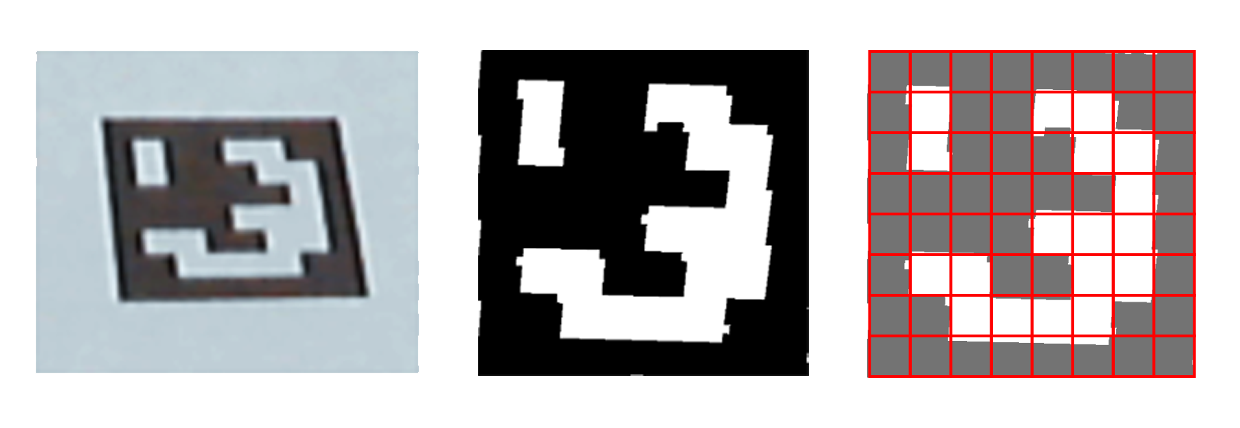
\includegraphics[width=0.7\textwidth]{figures/Fiducial.png}
    \caption{Candidate verification steps, from left to right: Detect candidate, transform of perspective, and lastly threshold based extraction of bits}\label{fig:fiducial}
\end{figure}

An experiment carried out in 2004 showed that using tracking systems based on a fiducial marker is reliable in a max range of app. 50-70 cm depending on the camera angle, after which the accuracy in tracking starts to suffer, which however can be accommodated by using more markers at different locations \cite{Abawi et al.}. However, this instability means that fiducial markers becomes impractical for distant tracking.


\subsubsection{Advanced Marker and NFT Tracking Systems}
Marker based tracking systems with or without a custom-made marker, named advanced marker tracking and natural feature tracking (NFT) respectively, involves image recognition. However, for an uncontrolled context like the ever changeable outdoors with its varying weather it is hard to calibrate the environment, insert landmarks, control lighting, and confine the operating range in order to facilitate tracking. Yet systems based on computer vision try to accommodate these obstacles. Computer vision has one or more optical sensors i.e. cameras continuously stream data that undergoes some image processing utilising natural features such as edges, corners, or texture patches extracted from the acquired camera images \cite{Barandiaram2010} \cite{Maidi2011}. 

Various approaches exist for marker based tracking based on computer vision. Some of the more commonly used approaches to realise AR dedicated to mobile applications is named SURF (Scale Invariant Feature Transform) and SIFT (Speeded Up Robust Features). Of these the SURF approach computes the fastest due to it using box filter techniques to compute a scale-space representation and first and second order differential operators \cite{Oyallon et al.}. Both of these methods, however, likewise track by using \textit{points of interest} and \textit{local invariant descriptors}. The latter is used to uniquely identify points of interest and match them, which can be done during various disruptive conditions. This can for instance be modifications in scale, rotation, illumination, or noise \cite{Maidi et al.}.

Overall  the SURF algorithm works through two consecutive steps. First step is \textit{feature detection}. Through this step candidates for the interest points are chosen. If their response is above a given threshold the candidate is validated afterwards. \cite{Oyallon et al.}. Next step is \textit{feature description}. The purpose of this step is to construct a descriptor of the neighborhood for each point of interest. \cite{Oyallon et al.} Lastly, to perform the image matching task, local descriptors from several images are matched, having them compared by computing the Euclidean distance between the potential matching pairs. To reduce mismatches a nearest-neighbor distance-ratio criterion is used \cite{Oyallon et al.} 


\begin{figure}[h!]
    \centering
    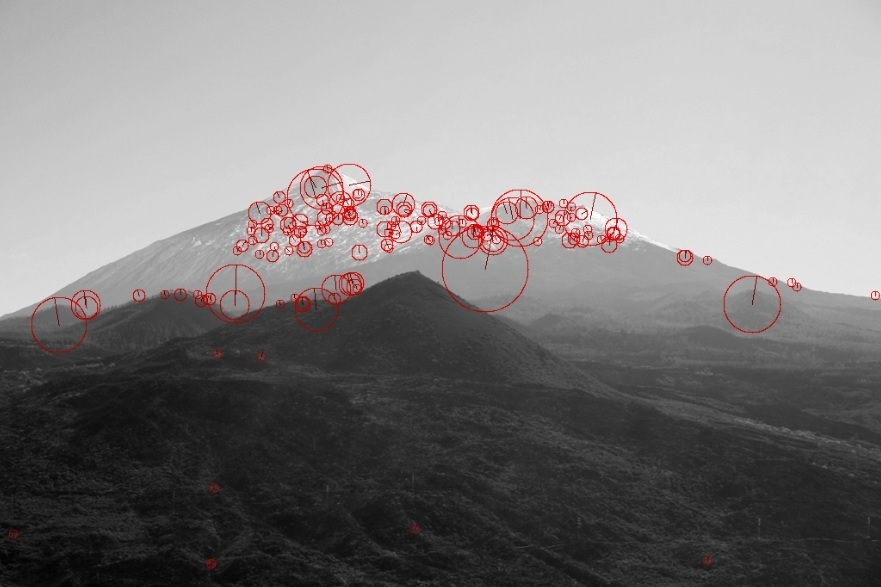
\includegraphics[width=0.7\textwidth]{figures/SURF.jpg}
    \caption{Image matching using the SURF algorithm}\label{fig:SURF}
\end{figure}

Roughly explained the SIFT method on the other hand manages this by first creating an internal representation of the original image. Then the algorithm searches for interest points. This is used to find key points. Then the disadvantageous key points are eliminated e.g. edges and low contrast regions. The remaining key points are afterwards assigned an orientation. Further calculations are then done relative to this orientation. Lastly, another representation is generated which helps identify features in the image \cite{Sinha}.


\begin{figure}[h!]
    \centering
    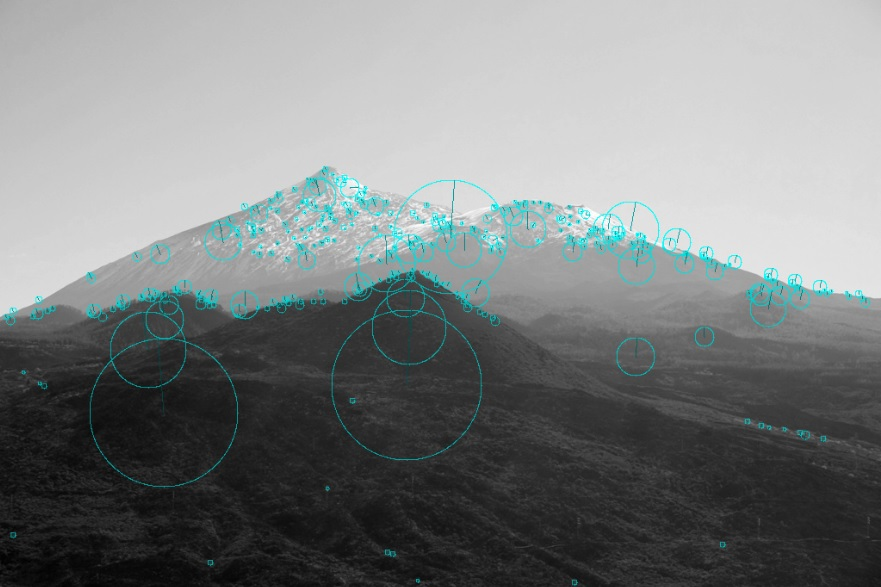
\includegraphics[width=0.75\textwidth]{figures/SIFT.jpg}
    \caption{Image matching using the SIFT algorithm}\label{fig:SIFT}
\end{figure}

The advantage of using one of the more advanced forms of tracking systems is that it imitates the process of the human perceptual system of vision in its way to perform pattern recognition from which to call background information \cite{Woodford}.

Based on the study of tracking systems it has been decided to use an advanced marker for the system developed for this project. The reason for this decision is to have the robustness in outdoor environments provided by tracking through computer vision while keeping the control which a marker provides. Furthermore this has been decided upon in order to avoid the limitations in accuracy concerning range and matching of the artificial world with the real world, troubles occurring by respectively using a fiducial based tracking system or location and orientation based tracking system.


\section{State of the Art}
Augmented reality can be used to various ends. The game Pokémon Go, which was released in the summer of 2016, includes an optional AR feature \cite{Pokemon}. However, AR has also been utilised for tourism. While a majority of AR solutions for tourists are scientific prototypes, a few commercial products are available for mobile smartphones. Using apps such as Wikitude, users can experience several different types of AR experiences, as developers are able to upload their AR project to the platform. The app uses different input methods to load the AR experiences, such as GPS location, images, and QR-codes \cite{Wikitude}. It primarily functions as a platform for AR advertisements or similar commercial products. The Yelp app, dedicated to reading and writing reviews of local restaurants, has an optional feature called \textit{monocle}. This allows users to see the average rating of nearby restaurants based on location \cite{Yelp}. A downside to this feature is that depending on the density of nearby restaurants, the screen may get quite cluttered, as can be seen in Figure \ref{fig:yelp}.\pagebreak

\begin{figure}[h!]
    \centering
    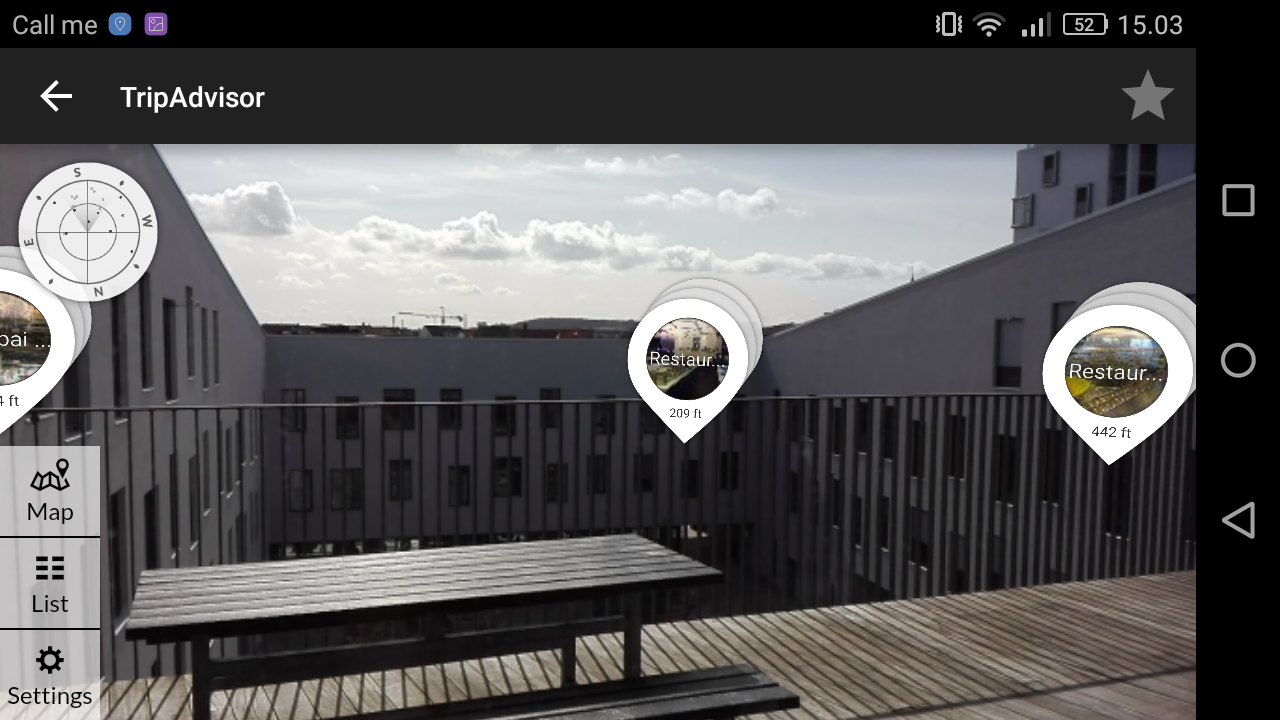
\includegraphics[width=\textwidth]{figures/wikitude.png}
    \caption{Screenshot of the Wikitude app, as utilised by Tripadvisor}\label{fig:wikitude}
\end{figure}
\hfill
\begin{figure}[h!]
    \centering
    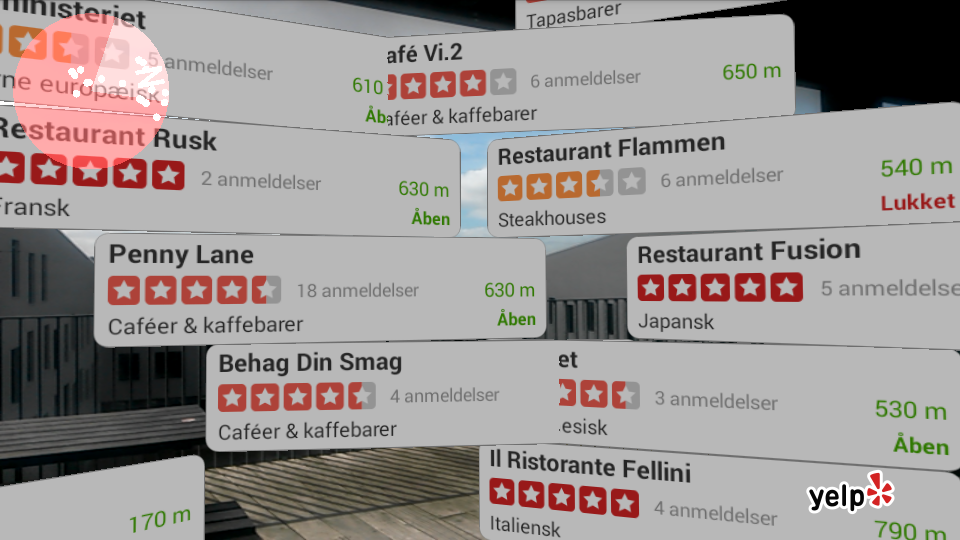
\includegraphics[width=\textwidth]{figures/yelp.png}
    \caption{Screenshot of the Yelp monocle feature}\label{fig:yelp}
\end{figure}

\pagebreak

\begin{wrapfigure}{l}{0.4\textwidth}
\centering
        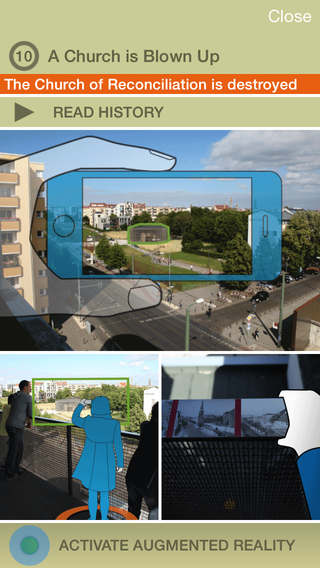
\includegraphics[width=0.4\textwidth]{figures/berlinwall.jpeg}
        \caption{The Berlin Wall Augmented app \cite{Hardenberg}}\label{fig:berlin}
\end{wrapfigure}

For examples of existing apps that have similar intend as the goal of this project are to be mentioned \textit{Timetraveler The Berlin Wall Augmented}, which as the developer describes it themselves: “transforms your mobile device into a window to the past.” \cite{Hardenberg}. This app guides the user to miscellaneous historic locations along the Berlin Wall showcasing how the specific site looked like shortly after the wall was built \cite{Hardenberg}, done by either an overlaying image or short video clip e.g. the crumbling of a church.

Another app is \textit{Streetmuseum} developed by Brothers and Sisters Creative Ltd on request from Museum of London. When the user holds up their camera this app lets them see an older version of London by adding an image as overlay covering the section of the present day street that the image represent, thereby offering “a window through time” \cite{Brothers}.

The research described in this chapter has covered the most important bases for this project, and based on it the research questions can now start being answered. The procedure for this will begin in the next chapter, where the design for the final prototype also is described.

\begin{figure}[h!]
    \centering
    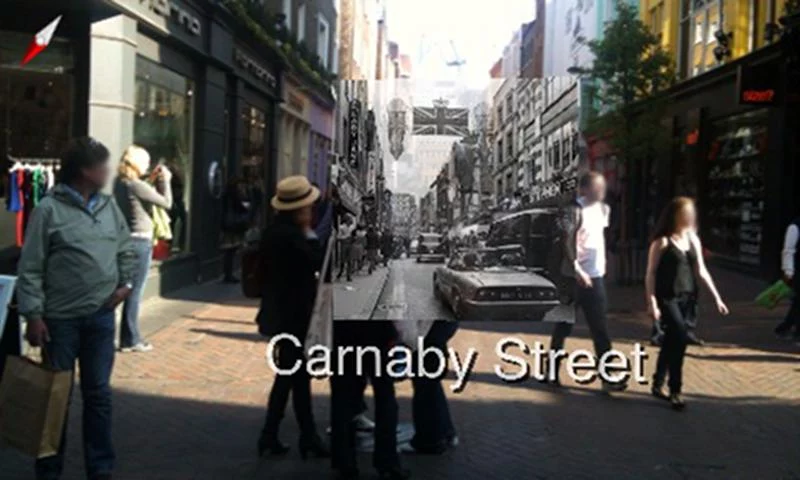
\includegraphics[width=0.75\textwidth]{figures/Streetmuseum.png}
    \caption{Screenshot of the Street Museum app \cite{Brothers}}\label{fig:streetmuseum}
\end{figure}

%I am just commenting this out in case we need it
%Here is equation~\eqref{eq:esun}:

%\begin{equation}
%\label{eq:esun}
%E_{sun} = (\vec{n} \cdot \vec{s}) \times \_E_{sun}
%\end{equation}